\documentclass{llncs}
\usepackage{graphicx}
\usepackage{url}
\usepackage{amsmath}
\usepackage{hyperref}
\begin{document}
\title{Analizarea și Îmbunătățirea Performanței MiniSat în Rezolvarea Problemei SAT \\ -Versiune draft- }
\author{Versiunea draft}
\author{Arpad-Adrian Precup, Elber Da, Szopuch Denis, Radu Bogdan}
\institute{
    Universitatea de Vest din Timișoara,\\
  Inginerie Software\\
    \email{} 
}

\maketitle

% \begin{abstract}
% Acest proiect explorează procesul de instalare și rulare al MiniSat, un SAT solver complet și de înaltă performanță, pe diferite sisteme de operare (Windows 10, Linux și o mașină virtuală cu Ubuntu). Problema SAT (satisfiabilitatea formulelor logice) este una dintre cele mai importante în informatică, având numeroase aplicații în domenii precum verificarea formală, inteligența artificială și teoria complexității. Proiectul documentează pașii de instalare și configurare a MiniSat, provocările întâmpinate în setările de debugging și compilare, precum și soluțiile aplicate pentru a obține o rulare funcțională a aplicației în medii de dezvoltare diferite.

% \keywords{MiniSat · SAT Solver · Instalare · Debugging ·}
% \end{abstract}

\begin{abstract}
SAT (problema satisfiabilității propoziționale) este una dintre cele mai importante și provocatoare probleme în informatică, având numeroase aplicații în domenii precum verificarea formală, inteligența artificială și teoria complexității. Aceasta se referă la a determina dacă există o interpretare care să satisfacă o formulă booleană dată. Acest proiect explorează procesul de instalare și rulare al MiniSat, un SAT solver complet și de înaltă performanță, pe diferite sisteme de operare: Windows 10, o mașină virtuală ce rulează Pop!\_OS (distribuție de Linux) și o mașină virtuală ce rulează Ubuntu.  Proiectul documentează pașii de instalare și configurare a MiniSat, provocările întâmpinate de-a lungul utilizării acestuia, de la configurare până la debugging, precum și soluțiile folosite pentru a obține o rulare funcțională a aplicației în medii de dezvoltare diferite.

\keywords{MiniSat · SAT Solver · Benchmark · Code analysis ·}
\end{abstract}

\newpage

\section{Introducere}

Problema satisfiabilității, cunoscută sub acronimul SAT, este o problemă esențială în teoria complexității computaționale, fiind prima problemă demonstrată ca fiind NP-completă, prin intermediul teoremei Cook-Levin\cite{ref_Cook_Levin_Theorem}. Aceasta constă în determinarea unei atriburi de adevăr pentru variabilele unei expresii logice astfel încât întreaga expresie să fie satisfăcută. Soluționarea problemelor SAT a devenit fundamentală într-o varietate de aplicații, inclusiv verificarea formală a software-ului și hardware-ului, inteligența artificială, probleme de optimizarea și bioinformatică.

MiniSat este un SAT solver disponibil public sub formă de repository pe GitHub\cite{ref_MiniSat_Original_Repository}. A fost creat cu scopul de a ajuta la introducerea de noi membrii în comunitatea SAT prin furnizarea unui SAT solver de dimensiuni reduse (dar eficient) și documentat. Cu toate că are dimensiuni reduse, MiniSat este un SAT solver complet și, cel puțin pentru data apariției sale în 2003, suportă toate funcționalitățile de ultimă oră are solverelor, precum: învățare bazată pe conflicte, backtracking bazat pe conflicte și two-literal watch scheme\cite{ref_MiniSat_home_page}. MiniSat are la bază algoritmul CDCL (Conflict-Driven Clause Learning), care este eficientizat prin diferite strategii, spre exemplu simplificarea clauzelor înainte de a începe procesul de rezolvare CDCL și aplicarea diferitelor euristici, precum luby restarts\cite{ref_luby_restart}. Dezvoltatorii MiniSat pun la dispoziție și diferite documente de documentație, care să ajute noii utilizatori și dezvoltatori să înteleagă felul în care MiniSat funcționează\cite{ref_MiniSat_docs}.

Acest proiect urmărește să documenteze procesul de instalare și configurare a MiniSat pe diverse platforme, punând accent pe provocările întâmpinate pe Windows și Linux, inclusiv rularea în mod debugging. De asemenea, include soluții pentru configurarea mediului de dezvoltare Visual Studio Code (VSCode), astfel încât să permită rularea și testarea programului într-un mod flexibil și reproductibil. Această lucrare va contribui la îmbunătățirea accesului la documentație pentru dezvoltatori și cercetători interesați de utilizarea MiniSat pe diferite platforme.

% \section{Descrierea Problemei SAT}

% Problema satisfiabilității, cunoscută sub numele de SAT, constă în determinarea valorilor de adevăr pentru variabilele unei expresii logice astfel încât întreaga expresie să fie satisfăcută, adică evaluată ca adevărată. În limbajul logicii propoziționale, o expresie este satisfiabilă dacă există o atribuire a valorilor variabilelor sale care face întreaga expresie să fie adevărată. Această problemă are o importanță majoră în teoria complexității deoarece este prima problemă cunoscută ca fiind NP-completă, fiind astfel esențială în clasificarea și înțelegerea problemelor computaționale complexe.

% Algoritmii utilizați pentru rezolvarea problemelor SAT includ tehnici diverse, cei mai reprezentativi fiind algoritmul DPLL și tehnica CDCL. Algoritmul DPLL (Davis-Putnam-Logemann-Loveland) utilizează tehnici de căutare recursivă, reducând treptat problema prin atribuiri succesive ale variabilelor și eliminarea condițiilor imposibile. CDCL (Conflict-Driven Clause Learning) este o optimizare a DPLL, care învață din conflictele întâlnite în timpul căutării soluției, reducând astfel numărul de căi explorate.

% Aplicațiile problemelor SAT sunt vaste și acoperă domenii variate, de la verificarea formală a corectitudinii sistemelor software și hardware până la inteligența artificială și bioinformatică. MiniSat, fiind un solver SAT foarte eficient, este utilizat adesea pentru a testa diverse benchmark-uri SAT și pentru a valida probleme complexe în cercetare și dezvoltare.

% \section{Problema SAT din perspectiva unui SAT solver}

\newpage

\section{Instalare MiniSat}

\subsection{Instalare pe Windows 10}

Pentru a instala MiniSat pe Windows 10, urmăm câțiva pași ce implică descărcarea codului sursă și configurarea unui mediu de dezvoltare compatibil. MiniSat este un proiect scris în C++, astfel că vom folosi Visual Studio Code sau un IDE similar pentru a permite compilarea și rularea codului C++. Este necesară instalarea MinGW, o suită de unelte care aduce funcționalitățile GNU Compiler Collection (GCC) pe Windows. Pașii necesari:
\begin{enumerate}
    \item Descărcăm codul sursă MiniSat de pe GitHub-ul oficial al proiectului\cite{ref_MiniSat_Original_Repository}.
    \item Instalăm MinGW pentru a putea compila codul C++.
    \item În timpul instalării am întâmpinat erori legate de tipizare strictă; astfel, a fost necesar să folosim opțiunea `CXXFLAGS="-fpermissive"` pentru a ignora aceste erori și a permite compilarea.
\end{enumerate}

\subsection{Instalare pe mașină virtuală ce rulează Pop!\_OS}

Instalarea MiniSat pe un sistem Linux este relativ simplă, datorită accesibilității librăriilor necesare și a suportului nativ pentru GNU Compiler Collection (GCC). Procesul se realizează prin terminal și implică actualizarea sistemului, descărcarea codului sursă, compilarea și rularea acestuia.

\begin{enumerate}
    \item Actualizăm lista de pachete și instalăm dependențele necesare.
    \item Descărcăm și compilăm codul MiniSat din repo-ul oficial.
    \item Pentru a compila cu succes a fost necesară utilizarea `CXXFLAGS="-fpermissive"`, fără de care procesul întâmpina erori de tipizare strictă.
    \item Pentru a putea face debugging, mediul de lucru trebuie configurat. Astfel, pentru Visual Studio Code trebuie creat un fișier `launch.json`, care permite rularea în modul debugging. Structura acestui fișier este exemplificată în secțiunea de README a repository-ului echipei noastre\cite{ref_MiniSat_our_fork}.
\end{enumerate}

\subsection{Instalare pe o Mașină Virtuală ce rulează Ubuntu}
\begin{enumerate}
    \item Deschidem terminalul și actualizăm pachetele sistemului cu comanda: "sudo apt update \&\& sudo apt upgrade".
    \item Instalăm dependențele necesare pentru compilare: "sudo apt install g++ make git"
    \item Clonăm codul sursă al MiniSat de pe GitHub: "git clone https://github.com/niklasso/minisat.git"
    \item Accesăm directorul minisat: "cd minisat" și compilăm MiniSat folosind: "sudo make CXXFLAGS="-fpermissive""
    \item Verificăm instalarea rulând: "./minisat"
\end{enumerate}

\section{Provocări Întâmpinate}

\subsection{Instalarea pe Windows}

Instalarea MiniSat pe Windows a întâmpinat mai multe provocări, în special din cauza diferențelor dintre compilatorul Windows și cerințele stricte de tipizare din codul sursă al MiniSat. Am utilizat flag-ul `-fpermissive` pentru a permite compilatorului să ignore aceste diferențe și să accepte codul.

\subsection{Rularea în Mod Debugging}

Pentru a permite debugging-ul în cea mai utilă formă, a fost necesară setarea opțiunii `CXXFLAGS = -fpermissive -g -O0`. Flag-ul `-g` este folosit pentru a specifica compiler-ului să includă informații pentru debugging în codul compilat. Astfel, putem folosi metodele de debugging (spre exemplu `step over`, `step into`) ca și cum am executa codul sursă și nu fișierele binare rezultate prin compilare. De asemenea, flag-ul `-O0` specifică compiler-ului nivelul de optimizare pe care acesta sa îl realizeze (adică să nu se realizez nici o optimizare a codului la compile time, tocmai pentru a putea parcurge codul în modul de depanare). Am adăugat toate aceste informații în fișierul de README al proiectului nostru pe GitHub\cite{ref_MiniSat_our_fork}

\subsection{Crearea fișierului launch.json în VSCode}

Pentru rularea MiniSat în Visual Studio Code, a fost necesară configurarea unui fișier `launch.json` specific, astfel încât MiniSat să fie accesibil prin extensia de C++ debugging din VSCode, această extensie oferind suport pentru testare și analiză interactivă. Fișierul de input pentru MiniSat este specificat ca parametru în acest fișier. Un aspect important este ca fișierul ales ca input să fie disponibil pentru operații de citire. Acest lucru se poate realiza cu ajutorul rulării comenzii \texttt{chmod 777 <fisier\_input>} înainte de a rula programul în mod debugging.

\section{Benchmarks}

Benchmark-urile utilizate pentru teste au fost preluate din competiția internațională SAT Competition 2024\cite{ref_SAT_Competition_home_page}.
Familia selectată este \texttt{Coloring}, care constă în probleme de colorare a grafurilor, reprezentate în format DIMACS CNF.
\subsection{Mediul de Execuție}
\subsection*{Hardware}
\begin{itemize}
    \item \textbf{Procesor:} 11th Gen Intel\textregistered\ Core\texttrademark\ i3-1115G4 @ 3.00 GHz.
    \item \textbf{Memorie RAM:} 8 GB (7.80 GB utilizabili).
    \item \textbf{Stocare:} SSD Samsung 970 EVO Plus, 1TB, NVMe, M.2.
    \item \textbf{Grafică:} Procesor grafic integrat Intel\textregistered\ UHD Graphics.
    \item \textbf{Arhitectură:} Sistem pe 64 de biți.
\end{itemize}

\subsection*{Software}
\begin{itemize}
    \item \textbf{Sistem de operare:} Windows 11 Home (versiunea 24H2) cu Ubuntu 24.04.1 LTS (prin WSL).
    \item \textbf{Solver SAT:} MiniSAT, versiunea preluată din repository-ul oficial.
\end{itemize}


\subsection{Rezultatele Testelor}

\begin{table}[h!]
    \centering
    \begin{tabular}{|l|c|c|}
    \hline
    \textbf{Coloring} & \textbf{Time (s, h)} & \textbf{Result} \\ \hline
    18c0eb461bda29214bd43b84199a3b61-cliquecolouring\_n31\_k5\_c4.sanitized & 34624.8 s (9 h 37 m) & INDETERMINATE \\ \hline
    67c533489a498495525efee429340958-cliquecolouring\_n15\_k9\_c8.sanitized & 74838.0 s (20 h 48 m) & INDETERMINATE \\ \hline
    973d699ec01b88da869233a79aaa1912-cliquecolouring\_n13\_k9\_c8.sanitized & 27204.1 s (7 h 33 m) & INDETERMINATE \\ \hline
    768956cc8d1f2d18ae1929f6bb26557a-cliquecolouring\_n13\_k8\_c7.sanitized & 30714.0 s (8 h 32 m) & INDETERMINATE \\ \hline
    ac347c21ca0759079c0be9a758e4e924-cliquecolouring\_n41\_k5\_c4.sanitized & 16077.5 s (4 h 28 m) & INDETERMINATE \\ \hline
    b172b4c218f1e44e205575d2b51e82c4-Schur\_161\_5\_d38 & 30172.4 s (8 h 22 m) & INDETERMINATE \\ \hline
    bbfe2b27182d2ee7fefdb557f458ac9c-cliquecolouring\_n21\_k6\_c5.sanitized & 25784.5 s (7 h 10 m) & INDETERMINATE \\ \hline
    cdd131110acc861a5a01fae6c4936c91-6g\_6color\_366\_050\_04 & Unknown & KILLED \\ \hline
    \end{tabular}
    \vspace{0.2cm}
    \caption{Rezultatul rulării benchmark-urilor din familia \texttt{Coloring}}
    \label{tab1}
\end{table}

În repository-ul echipei noastre de GitHub\cite{ref_MiniSat_our_fork}, în folderul \texttt{benchmarks}, se pot vedea mai multe detalii despre rularea fiecăruia dintre teste, cum ar fi numărul de conflicte, numărul de restart-uri, numărul de decizii luate sau memoria folosită.


\subsection{Observații}
\begin{itemize}
    \item În cadrul executării aplicației, s-au utilizat \textbf{1 GB RAM} dintr-un total de \textbf{8 GB}, ceea ce reprezintă aproximativ \textbf{12.5\%} din memoria disponibilă.
    \item Utilizarea procesorului (\textbf{CPU}) a fost de \textbf{36\%} pe parcursul execuției aplicației.
        \item Având în vedere că sistemul nu prezintă un nivel ridicat de performanță, la testul final realizat cu MiniSat, fișierul a avut o dimensiune semnificativă, astfel încât procesul a fost \textbf{întrerupt (KILLED)}, iar rezultatele nu au fost nici \textbf{UNSAT}, \textbf{SAT} sau \textbf{INDETERMINATE}.

\end{itemize}




\section{Codul Minisat}
\subsection{Structura fizică}
Proiectul MiniSat are următoare structură:
\begin{enumerate}
    \item \texttt{minisat/mtl/} - reprezintă Mini Template Library-ul asociat MiniSat. Conține diferite structuri de date generice care fac posibilă utilizarea MiniSat fără nevoia altor dependințe. În acest directory se găsesc, spre exemplu, implementări pentru structuri de date precum: Maps, cozi și vectori.

    \item \texttt{minisat/utils/} - conține helpere pentru cod. Spre exemplu, aici se găsesc metodele folosite pentru a interacționa cu sistemul I/O al mașinii pe care MiniSat este rulat și metode generice de parsat text, de exemplu: trecerea peste spațiile albe, trecerea peste o linie.

    \item \texttt{minisat/core/} - Versiunea core a MiniSat. Cu ajutorul metodelor și structurilor de date prezente în fișierele anterior menționate, aici are loc procesul de SAT solving. Aceasta este versiunea asupra căreia ne-am concentrat atenția (precizăm acest lucru deoarece există și o versiune cu mai multe îmbunătățiri, versiunea \hyperref[item:simp]{\texttt{simp}}).
    \begin{enumerate}
        \item \texttt{Dimacs.h} - Un fișier de tip header, care conține trei metode: \textbf{parse\_DIMACS}, \textbf{parse\_DIMACS\_main} și \textbf{readClause}. 
Dintre acestea, doar metoda \textbf{parse\_DIMACS} este apelată din exteriorul acestui fișier, aceasta fiind apelată din Main.cc pentru a insera problema (care este reprezentată într-un fișier text al cărui conținut trebuie să respecte formatul DIMACS) în Solver.
        \item \texttt{Main.cc} - Punctul de intrare în program. Acesta acceptă diferiți parametrii care pot fi utilizați pentru a particulariza execuția codului. Spre exemplu, prin folosirea parametrului \textbf{"verb"} pot fi selectate trei nivele de verbozitate, care modifică numărul de log-uri afișate pe parcursul rulării programului. 
Alți parametrii care pot fi setați: limită de timp pentru rulare (folosind parametrul \textbf{"cpu\_lim\"}), limită memorie folosită (folosind parametrul \textbf{"mem\_lim"}).
        \item \texttt{Solver.cc} - Conține codul pentru Solver. Include metode care crează noi variabile, adaugă clauze și rezolvă problema. Conține de asemenea și diferiți membrii precum modelul, acesta reprezentând o soluție a problemei, dacă aceasta a fost găsită.
        \item \texttt{Solver.h} - header-ul pentru clasa Solver.
        \item \texttt{SolverTypes.h} - Fișier header care conține definiția mai multor tipuri de date folosite de către Solver, printre care clasa \textbf{Clause} și struct-ul \textbf{Lit}. Aceste structuri de date sunt prezentate detaliat în secțiunea \hyperref[sec:data_structures]{\texttt{Structuri de date}}.
    \end{enumerate}
    \item \texttt{minisat/simp/} - Un solver extins care are capabilități pentru aplicarea de simplificări, fapt care duce la o performață mai bună. Această versiune este cea compilată implicit când se execută comanda \texttt{make} în terminal. Dacă se dorește compilarea versiunii core, este nevoie de rularea comenzii \texttt{make cr}.
    \label{item:simp}
\end{enumerate}

\subsection{Structura arhitecturală}
Componenta principală arhitecturală o reprezintă clasa \textbf{Solver}. Odată inserată problema în solver (folosind metoda \textbf{parse\_DIMACS}), acesta este capabil de a o rezolva prin intermediul metodei \textbf{solve\_}. Informații amănunțite despre cum funcționează metoda \textbf{solve\_} sunt disponibile în secțiunea dedicată \hyperref[sec:metode_remarcabile]{\texttt{metodelor remarcabile}}.

La nivel de diagramă de secvență, fluxul de date, de la rulare MiniSat din terminal până la afișarea output-ului, este următorul:

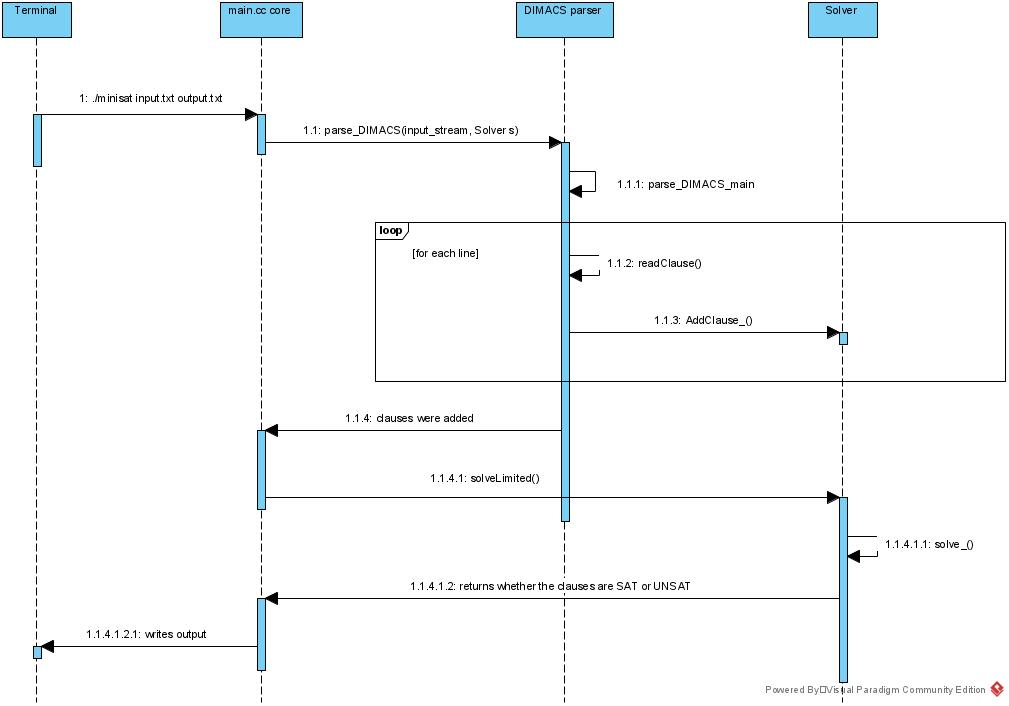
\includegraphics[width=1\textwidth]{resources/Minisat_main_sequence_diagram.jpg}

\subsection{Structuri de date}
\label{sec:data_structures}
% Prezinta cateva dintre structurile de date folosite si cum sunt folosite: ex. Lit
Datorită naturii problemei abordate de MiniSat, au fost declarate mai multe tipuri speciale de structuri de date peste care vom trece în această secțiune.

\begin{itemize}
    \item \textbf{Var} - este un alias pentru un număr întreg (integer). Variabilele trebuie alese de la 0 la N pentru a putea fi folosite ca indecși în vectori. Totodată, se declară și o instanță specială de tipul \textbf{Var} care reprezintă o variabilă neasignată, care are valoare -1. Aceste variabile reprezintă fiecare literal parsat din fișierul de input, cu o mică ajustare: variabilele de tip \textbf{Var}, fiind folosite ca indecși de vectori nu pot avea valori negative. De asemenea, trebuie să înceapă de la valoarea 0. Având în vedere că în formatul DIMACS literalii încep de la valoare absolută 1, valoare \textbf{Var} asociată se calculează prin decrementarea valorii absolute a literalului. Astfel, spre exemplu, dacă literalul parsat este "-1", valoare \textbf{Var} asociată este 0.
    \\
    \item \textbf{Lit} - este un struct care, conținând o singură valoare de tip integer, este capabil să encodeze un literal cu tot cu semnul asociat, folosindu-se de semnul literalului parsat și de valoarea \textbf{Var} asociată acestuia. Acest lucru este făcut posibil prin modul ingenios prin care valoarea din struct-ul \textbf{Lit} este calculată. Aceasta este calculată ca fiind dublul valorii \textbf{Var} asociate la care se adaugă 1 daca semnul literalului este negativ. Astfel, fiecărei posibile variabile \textbf{Var} îi sunt asociate două valori: \texttt{2 * var} și \texttt{2 * var + 1} (dacă semnul literalului este negativ).
    
    Așadar se ajunge ca numărul întreg stocat în \textbf{Lit} să aibă encodat pe cel mai puțin semnificant bit valoare semnului, iar pe restul de biți valoarea \textbf{Var} de la care provine. \\ Exemplu: Dacă literalul parsat este -7, atunci \textbf{Var}-ul asociat este 6. Luând în considerare și semnul literalului, variabila stocată în \textbf{Lit} va fi 13 (6 * 2 + 1). în reprezentare binară 13 este 1101, ultimul bit (1) reprezentând faptul că literalul este negat, iar restul reprezentând valoare \textbf{Var} asociată 0b110 = 6
    \\
    \item \textbf{Clause} - este o clasă care reprezintă o clauză. Conține un vector de \textbf{Lit} și diferite câmpuri care stochează date despre clauză cum ar fi dacă a fost învățată sau dimensiunea acesteia.
    \\
    \item \textbf{VMap} - o structură de date folosită în multe câmpuri din clasa Solver pentru a stoca date de tip \texttt{cheie -> valoare}, unde cheia este de tip \textbf{Var}. Exemple de astfel de câmpuri în solver sunt: \textbf{assigns} (stochează asignările curente pentru fiecare variabilă) și \textbf{polarity} (stochează polaritatea preferată pentru fiecare variabilă).   
\end{itemize}

\subsection{Metode remarcabile}
\label{sec:metode_remarcabile}

În această secțiune sunt prezentate câteva dintre metodele importante folosite pentru a rezolva problema satisfiabilității în MiniSat. Pentru metodele prezentate în această secțiune am realizat diagrame de activitate asociate, care pot fi vizualizate în directorul \texttt{diagrams} din repository-ul echipei noastre\cite{ref_MiniSat_our_fork}.
\subsubsection{Solve} - Metoda care implementează strategia de rezolvarea a problemei la nivelul cel mai superior. Această metoda folosește metoda \textbf{Search} și o restartează până când se ajunge la o concluzie sau "bugetul" (numărul de conflicte și propagări permise) este depășit.
\subsubsection{Search} - cea mai complexă procedură. În această procedură, variabilele sunt alese și le sunt atribuite valori (aceste asignări sunt stocate într-un vector de \textbf{Lit} numit \textbf{trail}. De asemenea, într-un vector de integers numit \textbf{trail\_lim} se rețin indecșii de la care încep nivele diferite de decizie în \textbf{trail}), până în momentul în care propagarea determină un conflict, punct în care se creează o clauză conflict care este adăugată Solver-ului ca și clauză învățată. Apoi se face backtracking, anulând asignările făcute la nivele mai înalte decât nivelul de la care a pornit conflictul (folosind informațiile din \textbf{trail} și \textbf{trail\_lim}). Odată procesul de backtracking terminat, se reîncepe cu procesul de propagare.

\begin{figure}[h]
\centering
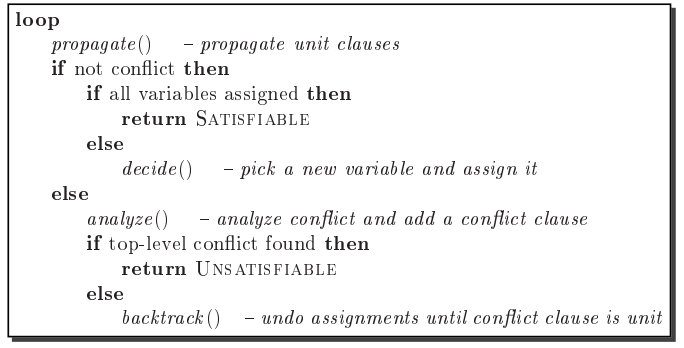
\includegraphics[width=1\textwidth]{resources/search_pseudocode.png}
\caption{\textbf{Pseudocod pentru metoda \textbf{Search}}\cite{ref_MiniSat_Extensible_SAT_Paper} }
\end{figure}

\subsubsection{Propagate} - Metoda care se ocupă de propagarea unității. 80\% din timpul de rulare MiniSat este datorat propagării, astfel această metodă poate fi considerată principală țintă când se dorește îmbunătățirea performanței\cite{ref_MiniSat_Extensible_SAT_Paper}. Această metoda folosește two-literal watch scheme pentru a eficientiza propagarea unitară.

\section{Repository GitHub}
Fork-ul nostru de MiniSat poate fi accesat la \href{https://github.com/aprecup14/minisat}{https://github.com/aprecup14/minisat} \cite{ref_MiniSat_our_fork}. Acesta conține pe lângă codul de MiniSat (căruia i-am actualizat părți din documentația scrisă sub formă de comentarii) următoarele foldere:
\begin{itemize}
    \item \texttt{Benchmarks} - fișier care conține rezultatele rulării benchmark-urilor. În acest fișier se pot observa două fișiere care corespund membrilor echipei care s-au ocupat de rularea testelor. În aceste fișiere se pot observa afișările care se produc în timpul rulării MiniSat. De asemenea, există și un fișier \texttt{Specs.txt} care precizează specificațiile mașinii care a rulat benchmark-urile.
    \item \texttt{Diagrams} - Acest fișier conține diagramele UML pe care le-am creat pentru a reprezenta diferite fluxuri de date în MiniSat. Pentru realizarea diagramelor am folosit \texttt{Visual Paradigm}.
    \item \texttt{Latex overleaf} - Fișier în care încărcăm codul sursă pentru documentul latex.
    \item \texttt{README.md} - Fișier pe care l-am actualizat cu diferite informații legate de cum trebuie rulat MiniSat. Spre exemplu, instrucțiuni pentru a putea rula MiniSat în mod debugging în \texttt{Visual Studio Code}.
\end{itemize}
\section{Responsabilități}
Fiecare membru al echipei a avut responsabilități:
\begin{itemize}
    \item \texttt{Arpad-Adrian Precup} - 
    \begin{itemize}
        \item Crearea mediului propice pentru a realiza comunicarea și lucrul în echipă. Crearea repository-ului de GitHub, crearea proiectului în Overleaf, adăugarea celorlalți membrii ai echipei ca și contribuitori la aceste proiecte. Adăugarea de foldere pentru încărcarea benchmark-urilor, diagramelor și a codului sursă latex în GitHub.
        \item Rularea MiniSat ca developer (folosind codul sursă). Rularea MiniSat în mod debugging pentru a observa fluxul de date.
        \item Înțelegerea modului de funcționare a MiniSat. Identificare utilizării algoritmului CDCL cu diferite ajustări/îmbunătățiri.
        \item Crearea documentației tehnice și a diferitelor diagrame UML.
        \item Redactat secțiune latex care prezintă cum funcționează codul MiniSat.
        \item Revizuit document latex și ajutat membrii echipei la nevoie.
\\
    \end{itemize}

    \item \texttt{Denis Szopuch}
    \begin{itemize}
        \item Redactat abstract și introducere care să explice contextul proiectului, tehnologiile utilizate și importanța acestuia.
        \item Scrierea unui rezumat clar și concis al proiectului, subliniind scopul și obiectivele.
        \item Instalare MiniSat.
        \item Crearea unui ghid pas cu pas pentru instalarea MiniSat, inclusiv cerințele și pașii necesari pentru a-l rula pe diferite platforme.
        \item Redactarea secțiunii de concluzii, sintetizând rezultatele obținute și impactul implementării.
        \\
    \end{itemize}

    \item \texttt{Elber Da}
    \begin{itemize}
        \item Instalare MiniSat.
        \item Rularea benchmark-ului de coloring
        \item Observarea și documentarea comportamentului MiniSat în timpul rulării benchmark-urilor.
        \item Redactarea secțiunii legată de benchmarks.
        \item Încărcarea rezultatelor benchmark-urilor pe GitHub.      
        \\
    \end{itemize}

    \item \texttt{Cristian Radu}
    \begin{itemize}
        \item Instalare MiniSat.
        \item Rularea benchmark-ului de coloring
        \item Observarea și documentarea comportamentului MiniSat în timpul rulării benchmark-urilor.
        \item Redactarea secțiunii legată de benchmarks.
        \item Încărcarea rezultatelor benchmark-urilor pe GitHub.
    \end{itemize}
\end{itemize}

    Pe lângă contribuțiile individuale, am păstrat legătura constant și am avut discuții despre stadiul sarcinilor fiecăruia prin intermediul unui grup de WhatsApp. Am avut de asemenea ședinte de lucru comune pe Google Meet prin care am conectat părțile lucrate individual de fiecare membru.

\section{Concluzii}

În cadrul acestui proiect, am investigat și utilizat MiniSat pentru a rezolva probleme SAT, utilizând o familie de probleme de benchmark din competiția SAT 2024\cite{ref_SAT_Competition_home_page} pentru a analiza performanța acestuia. De asemenea, versiunea draft a proiectului a avut ca scop familiarizarea cu MiniSat și înțelegerea algoritmilor de rezolvare a problemei SAT folosiți de MiniSat.

Am identificat principalul algoritm de rezolvare a problemei SAT folosit de MiniSat, CDCL (Conflict-Driven Clause Learning), care este implementat eficient în MiniSat, cu tehnici care îmbunătățesc performanța cum ar fi two-literal watch scheme și diferite euristici de resetare precum luby restarts. Aceste tehnici sunt esențiale pentru îmbunătățirea performanței MiniSat în probleme de satisfiabilitate, iar analiza detaliată a codului sursă ne-a permis să înțelegem cum aceste metode sunt integrate și optimizate. De asemenea, am identificat zonele unde MiniSat poate fi îmbunătățit, în special zona de propagare care ocupă 80\% din timpul de rulare al MiniSat\cite{ref_MiniSat_Extensible_SAT_Paper}.

Un aspect important al proiectului a fost experimentarea cu benchmark-uri SAT din competiția SAT 2024\cite{ref_SAT_Competition_home_page}. Rezultatele obținute au arătat performanțe bune ale MiniSat în rezolvarea unor instanțe de dimensiuni reduse, dar și provocări legate de timpul de execuție și eficiența în cazul unor formule extrem de mari sau complexe.

Provocările întâmpinate au inclus înțelegerea complexității codului sursă MiniSat și integrarea acestuia într-un mediu de testare eficient. De asemenea, documentația limitată sau învechită a fost o barieră în calea înțelegerii complete a tuturor funcționalităților MiniSat, ceea ce a făcut necesar un studiu suplimentar al literaturii de specialitate pentru a clarifica anumite concepte avansate.

În ansamblu, proiectul ne-a permis să aprofundăm cunoștințele teoretice legate de SAT solving și să ne dezvoltăm abilitățile practice de programare, analiză de performanță a software-ului și capacitățile de colaborare în echipă.


%
% ---- Bibliography ----
%
% BibTeX users should specify bibliography style 'splncs04'.
% References will then be sorted and formatted in the correct style.
%
% \bibliographystyle{splncs04}
% \bibliography{mybibliography}
%
\begin{thebibliography}{8}
\bibitem{ref_Cook_Levin_Theorem}
UBC Department of Computer Science, \url{https://www.cs.ubc.ca/~condon/cpsc506/handouts/Cook-Levin.pdf}
% , ultima accesare 2024/11/14

\bibitem{ref_MiniSat_Original_Repository}
Repository-ul oficial MiniSat, \url{https://github.com/niklasso/minisat}
% , ultima accesare 2024/10/30

\bibitem{ref_MiniSat_home_page}
MiniSat Home Page, \url{http://minisat.se/MiniSat.html}
% , ultima accesare 2024/11/17

\bibitem{ref_luby_restart}
Luby restart, \url{https://choco-solver.org/docs/solving/restarts/#luby}
% , ultima accesare 2024/11/17

\bibitem{ref_MiniSat_docs}
MiniSat documentation page, \url{http://minisat.se/Papers.html}
% , ultima accesare 2024/11/17

\bibitem{ref_MiniSat_our_fork}
Fork-ul nostru de MiniSat, \url{https://github.com/aprecup14/minisat}
% , ultima accesare 2024/11/17

\bibitem{ref_SAT_Competition_home_page}
SAT competition home page, \url{https://satcompetition.github.io/2024/}
% , ultima accesare 2024/11/17

\bibitem{ref_MiniSat_Extensible_SAT_Paper}
An Extensible SAT-solve paper, \url{http://minisat.se/downloads/MiniSat.pdf}
% , ultima accesare 2024/11/17
% \bibitem{ref_article1}
% Author, F.: Article title. Journal \textbf{2}(5), 99--110 (2016)

% \bibitem{ref_lncs1}
% Author, F., Author, S.: Title of a proceedings paper. In: Editor,
% F., Editor, S. (eds.) CONFERENCE 2016, LNCS, vol. 9999, pp. 1--13.
% Springer, Heidelberg (2016). \doi{10.10007/1234567890}

% \bibitem{ref_book1}
% Author, F., Author, S., Author, T.: Book title. 2nd edn. Publisher,
% Location (1999)

% \bibitem{ref_proc1}
% Author, A.-B.: Contribution title. In: 9th International Proceedings
% on Proceedings, pp. 1--2. Publisher, Location (2010)

% \bibitem{ref_url1}
% LNCS Homepage, \url{http://www.springer.com/lncs}, last accessed 2023/10/25
\end{thebibliography}
\end{document}